\section{Модель ресурса сборочной линии}
\indent В процессе создания оперативного плана, для получения адекватной оценки времени выполнения операции (набора операций) СПП необходимо ввести систему ограничений, которая будет отражать как ресурс, участвующий в операции может влиять на её время выполнения.
Это привело к созданию модели ресурсов накладывающей ограничения на выбор операции для расчета ядром имитационного моделирования.\\
\indent Каждый ресурс представляет из себя структуру данных, которая должна реализовывать три метода:

\begin{itemize}
	\item привязка операции к ресурсу;
	\item метод, осуществляющий проверку возможности выполнения данной операции ресурсом;
	\item метод, осуществляющий логику работы и в котором происходит изменение состояния данного ресурса.
\end{itemize}

\indent Привязка осуществляется в начале работы системы, что позволяет ресурсам манипулировать ядром имитационного моделирования разрешая или запрещая выбирать привязанные к ним операции для расчета, что может повлечь за собой изменение последовательности выполнения операций и, соответственно, расчетного времени выполнения набора операций.\\
\indent Проверка производится во время работы системы и именно здесь происходит отбор операций в соответствии с внутренним состоянием ресурса.\\
\indent Логика осуществляется при выборке операции ядром и для каждой вызывается два раза: чтобы отметить состояние ресурса в начале и в конце расчета операции.\\
\indent Одним из ресурсов является ресурс сборочной линии, который описывает несколько однотипных, то есть с одинаковым числом рабочих постов (заготовко-места, оснащенные соответствующим технологическим оборудованием и предназначенными для технического воздействия на заготовку для осуществления фиксированного перечня операций), физических сборочных линий.
Объединение нескольких сборочных линий в одну обуславливается упрощением взаимодействия с ядром имитационного моделирования, а также возможностью инкапсуляции реализации распределения наборов операций по сборочным линиям внутри ресурса.\\

\begin{figure}[hb!]
	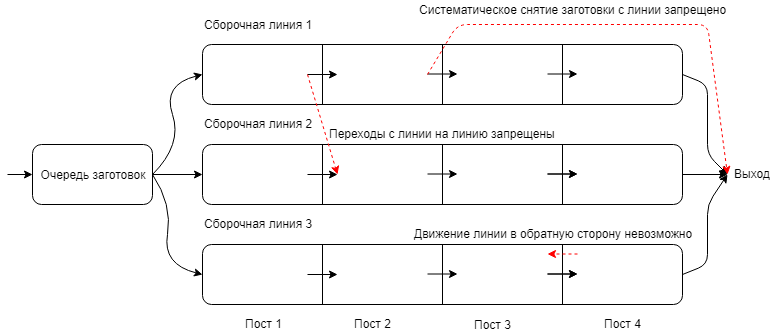
\includegraphics[width=\linewidth]{pics/assemblyMain.png}
	\caption{Схема ресурса с вариантами перемещения заготовки внутри}
	\label{fig:assemblyMain}
	% \centering
\end{figure}

\indent Главным предназначением данного ресурса является ограничение перемещения продукции (над которой производится набор операций).
С одной стороны ограничивается перемещение между сборочными линиями: к какой продукт был привязан, на той он и останется до окончания выполнения всех операций, которые относятся к данному продукту и привязаны к данной сборочной линии.
С другой - ограничивается и синхронизируется перемещение продукции между рабочими постами: продукт должен двигаться последовательно с поста на пост (см. \ref{fig:assemblyMain}).\\
\indent Основной сложностью реализации данного модуля является предложенная система ресурсов, которая является универсальной и позволяет реализовать логику любого ресурса, при этом усложняя реализацию каждого из них.
В данной реализации ресурса каждая из линий характеризуется временем начала текущего рабочего такта сборочной линии (время, в течение, которого заготовка пребывает на посту), текущим или максимальным временем рабочего такта и набором рабочих постов, каждый из которых описывается состоянием (выполняются работы, простаивает), временной меткой данного поста и продукцией, которая на данный момент находится на нем.
Также ресурс имеет информацию о привязке каждой операции каждой единицы продукции к какому-либо рабочему посту (без привязки к конкретной линии) сборочной линии, что дает возможность динамически распределять продукцию между линиями.\\
\indent Во время работы ядра имитационного моделирования на каждой итерации проверяется наличие привязки ресурсов ко всем доступным для выбора операциям и, при наличии таковых, осуществляется опрос каждого ресурса на то, накладывает ли он какое-либо ограничение на выбор данной операции в текущую итерацию.

\todo[inline]{блок-схема ресурсов}

% \todo[inline]{Подумать над формулировкой}
% Данная компонента является частью (или частной реализацией) модели ресурсов СПП и отражает поведение во времени продуктов на сборочной линии. Основная сложность данной компоненты в необходимости объединения нескольких сборочных линий со схожими параметрами в один ресурс, хранении их состояний, синхронизации между \todo{постами} и распределении \todo{входного потока продуктов} по линиям. Также, сложностью является сама модель ресурса, которая обеспечивает хорошую масштабируемость, но при этом требует времени на понимание и создание модулей.